\section*{Problem 8.2 - Receiver diversity, MRC, EGC and SC}
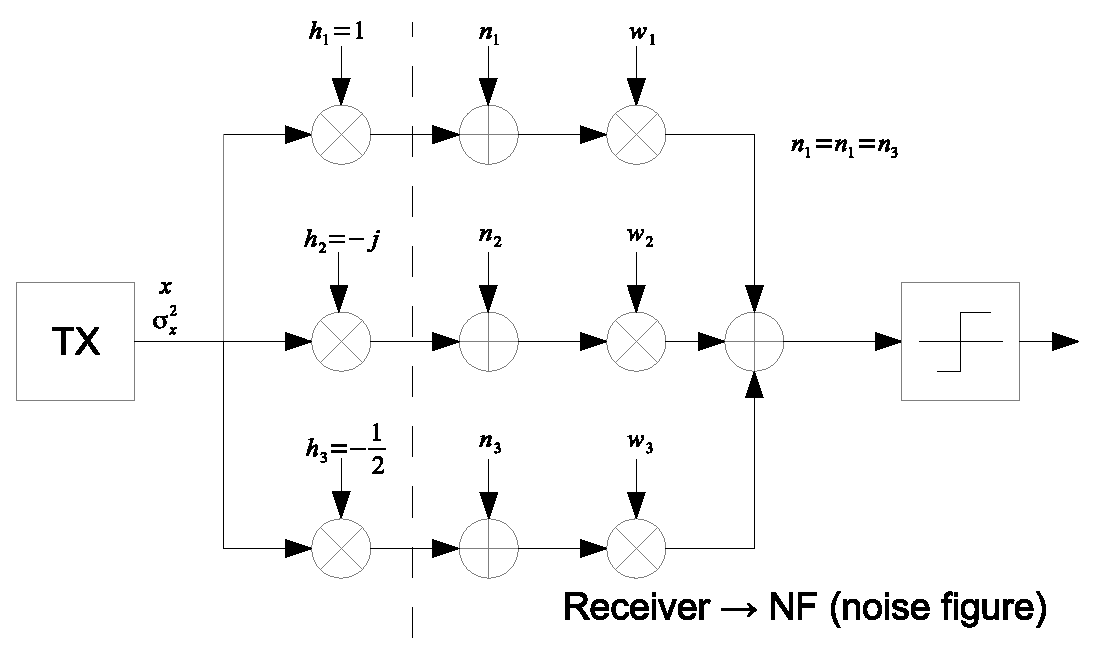
\includegraphics[width=1\textwidth]{MIMO_receiver.eps} \\
\subsection*{a)}
\begin{align*}
	\mathrm{MRC}\quad\rightarrow\quad & w_j =h_j^*\quad\forall j\in\{1,\ldots,N_R\} \\
	& w_1=1 \\
	& w_2=j \\
	& w_3=-\frac{1}{2} \\
	&\text{In order to have $w_j$ we need $h_j$ $\rightarrow$ channel estimation} \\
	\mathrm{EGC}\quad\rightarrow\quad & h_n=\left|h_n\right|e^{j\phi_n}\quad\Rightarrow\quad w_n=e^{j\phi_n} \\
	& h_1=1\quad\rightarrow\quad w_1=1 \\
	& h_2=-j\quad\rightarrow\quad w_2=j \\
	& h_3=-\frac{1}{2}\quad\rightarrow\quad w_3=e^{-j\pi}=-1
\end{align*}

\subsection*{b)}
\begin{align*}
	\mathrm{MRC:} & \quad\mathrm{SNR_{total}^{MRC}}=\frac{\sigma_x^2\left|\sum\limits_{n=1}^{N_R}h_nw_n\right|^2}{\sigma_n^2\sum\limits_{n=1}^{N_R}\left|w_n\right|^2} = \frac{\sigma_x^2\left|\sum\limits_{n=1}^{N_R}\left|h_n\right|e^{j\phi_n}\left|h_n\right|e^{-j\phi_n}\right|^2}{\sigma_n^2\sum\limits_{n=1}^{N_R}\left|h_n\right|^2}= \\
	& \qquad=\frac{\sigma_x^2}{\sigma_n^2}\left(\sum\limits_{n=1}^{N_R}\left|h_n\right|^2\right)=\frac{\sigma_x^2}{\sigma_n^2}\left(1+1+\frac{1}{4}\right) \\
	& \qquad\Rightarrow\boxed{\mathrm{SNR_{total}^{MRC}}=\frac{9}{4}\frac{\sigma_x^2}{\sigma_n^2}} \\
	\mathrm{EGC:} & \quad\mathrm{SNR_{total}^{EGC}}=\frac{\sigma_x^2\left|\sum\limits_{n=1}^{N_R}\left|h_n\right|e^{j\phi_n}e^{-j\phi_n}\right|^2}{\sigma_n^2\sum\limits_{n=1}^{N_R}\left|e^{-j\phi_n}\right|^2}= \\
	& \qquad=\frac{\sigma_x^2}{N_R\sigma_n^2}\left(\sum\limits_{n=1}^{N_R}\left|h_n\right|^2\right)=\frac{\sigma_x^2}{3\sigma_n^2}\left(1+1+\frac{1}{2}\right)^2 \\
	& \qquad\Rightarrow\boxed{\mathrm{SNR_{total}^{EGC}}=\frac{25}{12}\frac{\sigma_x^2}{\sigma_n^2}} \\
	\mathrm{SC:} & \quad\text{branch with max. SNR: } \hat{n}=\argmax_n\mathrm{SNR}_n\quad\rightarrow\quad\mathrm{SNR_{total}}=\mathrm{SNR}_{\hat{n}} \\
	& \quad\text{we need SNR estimation algorithm $\rightarrow$ e.g. pilots} \\
	& \qquad\mathrm{SNR}_1=\frac{\sigma_x^2\left|h_1\right|^2\left|w_1\right|^2}{\sigma_n^2\left|w_1\right|^2}=\frac{\sigma_x^2}{\sigma_n^2}\left|h_1\right|^2=\frac{\sigma_x^2}{\sigma_n^2} \\
	& \qquad\mathrm{SNR}_2=\frac{\sigma_x^2}{\sigma_n^2}\left|h_2\right|^2=\frac{\sigma_x^2}{\sigma_n^2} \\
	& \qquad\mathrm{SNR}_3=\frac{\sigma_x^2}{\sigma_n^2}\left|h_3\right|^2=\frac{1}{4}\frac{\sigma_x^2}{\sigma_n^2} \\
	& \quad\text{$\mathrm{SNR}_1$/$\mathrm{SNR}_2$ is the highest SNR, we select first branch} \\
	& \quad\rightarrow\quad\boxed{\mathrm{SNR_{total}^{SC}}=\mathrm{SNR}_1=\frac{\sigma_x^2}{\sigma_n^2}}
\end{align*}
\begin{align*}
	\left.
	\begin{aligned}
		\mathrm{MRC:} & \quad\mathrm{SNR_{total}^{MRC}}=\frac{4}{9}\frac{\sigma_x^2}{\sigma_n^2} \\
    \mathrm{EGC:} & \quad\mathrm{SNR_{total}^{EGC}}=\frac{25}{12}\frac{\sigma_x^2}{\sigma_n^2} \\
		\mathrm{SC:} & \quad\mathrm{SNR_{total}^{SC}}=\frac{\sigma_x^2}{\sigma_n^2}
  \end{aligned}
	\right\}
	\quad\boxed{\mathrm{SNR}^{MRC}\ge\mathrm{SNR}^{EGC}\ge\mathrm{SNR}^{SC}}
\end{align*}
